\documentclass[11pt,a4paper]{article}

% ============================================================================
% Packages
% ============================================================================
\usepackage[utf8]{inputenc}
\usepackage[T1]{fontenc}
\usepackage{lmodern}
\usepackage{amsmath,amssymb,amsfonts,amsthm}
\usepackage{graphicx}
\usepackage[dvipsnames,svgnames,x11names]{xcolor}
\usepackage{geometry}
\usepackage{booktabs}
\usepackage{fancyhdr}
\usepackage{hyperref}
\usepackage{tikz}
\usepackage{pgfplots}
\usepackage{float}
\usepackage{enumitem}
\usepackage{caption}
\usepackage{subcaption}
\usepackage{tabularx}
\usepackage{mathtools}
\usepackage{tcolorbox}
\usepackage{titlesec}
\usepackage{parskip}
\usepackage{epigraph}

\usetikzlibrary{arrows.meta,positioning,calc,decorations.pathmorphing,backgrounds,fit,shapes.geometric}
\pgfplotsset{compat=1.18}

\geometry{margin=2.5cm,top=2.8cm,bottom=2.8cm}

\newtheorem{theorem}{Theorem}[section]
\newtheorem{lemma}[theorem]{Lemma}
\newtheorem{definition}[theorem]{Definition}
\newtheorem{remark}[theorem]{Remark}

\tcbuselibrary{skins,breakable}

% ============================================================================
% Colors
% ============================================================================
\definecolor{quantumcyan}{HTML}{00D4FF}
\definecolor{quantumpurple}{HTML}{8B5CF6}
\definecolor{quantumgreen}{HTML}{10B981}
\definecolor{sectionblue}{HTML}{2563EB}
\definecolor{measured}{HTML}{059669}
\definecolor{hardcoded}{HTML}{D97706}
\definecolor{theoretical}{HTML}{7C3AED}
\definecolor{chalkboard}{HTML}{1A2332}

% Custom environments
\newtcolorbox{honesty}{
    colback=orange!5, colframe=orange!70!black,
    fonttitle=\bfseries\small, title={Data Honesty Note}, breakable
}

\newtcolorbox{blackboard}[1][]{
    colback=chalkboard!95!black, colframe=chalkboard,
    coltext=white, fonttitle=\bfseries\color{quantumcyan},
    title={#1}, breakable, arc=2mm
}

\newtcolorbox{susskindbox}[1][]{
    colback=blue!3, colframe=sectionblue!60,
    fonttitle=\bfseries\small\color{sectionblue},
    title={#1}, breakable
}

% ============================================================================
% Hyperref
% ============================================================================
\hypersetup{
    colorlinks=true, linkcolor=sectionblue, citecolor=quantumpurple, urlcolor=quantumcyan,
    pdftitle={The Theoretical Minimum for Blockchain Consensus},
    pdfauthor={Q-NarwhalKnight Research},
}

% ============================================================================
% Header/Footer
% ============================================================================
\pagestyle{fancy}
\fancyhf{}
\fancyhead[L]{\small\textcolor{gray}{The Theoretical Minimum for Blockchain Consensus}}
\fancyhead[R]{\small\textcolor{gray}{v3 --- April 2026}}
\fancyfoot[C]{\small\textcolor{gray}{\thepage}}
\renewcommand{\headrulewidth}{0.4pt}

\setlength{\epigraphwidth}{0.75\textwidth}

% ============================================================================
% Title
% ============================================================================
\title{%
\vspace{-1cm}
{\LARGE\textbf{The Theoretical Minimum\\for Blockchain Consensus}}\\[0.4cm]
{\large A Statistical Mechanics Framework for DAG-Knight,\\Explained from First Principles}\\[0.4cm]
{\normalsize\textcolor{gray}{With honest accounting of what we measure, what we assume,\\and what we don't know yet}}\\[0.3cm]
{\small\textcolor{sectionblue}{Revised after peer review by DeepSeek and ChatGPT}}
}

\author{%
\textbf{Q-NarwhalKnight Research}\\
\texttt{research@quillon.xyz}\\[0.2cm]
{\small Network: \texttt{mainnet-genesis} $\mid$ v10.2.8 $\mid$ 14,329,651 blocks $\mid$ 12 peers $\mid$ 47.9 days uptime}
}

\date{April 11, 2026 --- v3}

\begin{document}
\maketitle

\epigraph{``The best thing about physics is that it tells you when you're wrong. The worst thing about physics-inspired analogies is that they never do.''}{---Adapted, in the spirit of Susskind}

% ============================================================================
% Abstract
% ============================================================================
\begin{abstract}
We present an observability framework for DAG-Knight blockchain consensus that uses the language of statistical mechanics---Hamiltonians, temperature, phase diagrams, entropy, and diffusion---to organize network diagnostics into a coherent, quantitative picture. We are explicit about the epistemological status of every claim: one theorem is proven (the Ground State Correspondence), several formulas are testable quantitative models, and the rest is structural analogy. We validate against 14.3 million blocks on a live mainnet, present simulated stress scenarios, and catalog every measurement gap where hardcoded placeholders replace real data. The paper is written in an expository style inspired by Susskind's \emph{Theoretical Minimum}: we explain what each formula means, why we chose it, where it comes from, and where it fails. This is an engineering contribution dressed in physics notation---not a physics contribution. The physics notation is useful because it gives us additive decomposition (Hamiltonian), a single stress scalar (temperature), a visual operating envelope (phase diagram), and an information-theoretic measure of ambiguity (entropy). We use these tools honestly and invite the reader to hold us to that standard.
\end{abstract}

\tableofcontents
\newpage

% ============================================================================
% PART I: WHY PHYSICS NOTATION?
% ============================================================================
\part{Why Physics Notation for a Blockchain?}

% ============================================================================
% 1. The Problem
% ============================================================================
\section{The Problem: What Does ``Healthy'' Mean?}

Let's start with a concrete problem that every blockchain node operator faces. You're running a node. You look at the dashboard. You see:

\begin{itemize}
    \item Block height: 14,329,651
    \item Connected peers: 12
    \item Block rate: 3.46 blocks/second
\end{itemize}

Is the network healthy? You might say ``yes, it's producing blocks.'' But that's not enough. A network can produce blocks and still be:

\begin{itemize}
    \item \textbf{Slow to converge} --- nodes disagree on block ordering for too long.
    \item \textbf{Close to a security boundary} --- one more adversarial peer and consensus breaks.
    \item \textbf{Producing ambiguous orderings} --- multiple valid ways to order concurrent blocks.
    \item \textbf{Under subtle attack} --- an adversary maintaining ``normal'' metrics while slowly poisoning the DAG.
\end{itemize}

What you really want is a \emph{decomposition} of network health into independent, interpretable components. And you want a single number---a \emph{stress indicator}---that tells you ``this is fine'' or ``something is wrong.''

This is exactly what physicists do when they study complex systems. They decompose the system's state into energy terms (the Hamiltonian), define a single number that captures disorder (temperature), and draw phase diagrams showing where the system works and where it doesn't.

We're going to borrow that toolkit. Not because the blockchain is a physical system---it isn't. But because the mathematical structures are useful for exactly the same reason they're useful in physics: they give you a principled way to decompose, quantify, and visualize the state of a complex system.

% ============================================================================
% 2. What We're Not Claiming
% ============================================================================
\section{What We Are \emph{Not} Claiming}

Before we write a single equation, let's be clear about the epistemological status of this work. We classify every claim at one of three levels:

\begin{susskindbox}[Three Levels of Claims]
\begin{enumerate}
    \item \textbf{Exact Theorem} (\textcolor{measured}{$\blacksquare$}): A proven mathematical statement with explicit assumptions. We have exactly one of these---the Ground State Theorem (Section~\ref{sec:groundstate}), which proves that the Hamiltonian's minimum corresponds to the PHANTOM algorithm's output.

    \item \textbf{Quantitative Model} (\textcolor{hardcoded}{$\blacksquare$}): A formula that makes testable predictions. The effective temperature $T_{\text{eff}}$, the critical threshold $\kappa_c$, and the diffusion model are at this level. They could be \emph{wrong}---but they're wrong in a falsifiable way.

    \item \textbf{Structural Analogy} (\textcolor{theoretical}{$\blacksquare$}): Conceptual vocabulary borrowed from physics for intuition. ``Temperature,'' ``entropy,'' and ``phase transition'' are used at this level. They help organize thinking but don't imply the blockchain exhibits thermodynamic phenomena.
\end{enumerate}
\end{susskindbox}

The previous version of this paper (v1) was reviewed by DeepSeek and ChatGPT. Both rejected it, correctly identifying that we had blurred the lines between these levels---presenting structural analogies as if they were exact theorems, and hardcoded constants as if they were live measurements. This version fixes that.

\subsection{An Analogy for the Analogy}

Think of it this way. When economists talk about ``market temperature'' or ``economic entropy,'' nobody believes the stock market is literally at 300 Kelvin. But the language is useful: high ``temperature'' means high volatility; low ``entropy'' means concentrated positions. The math of statistical mechanics---Boltzmann distributions, partition functions, free energy---turns out to be the right formalism for many systems that have nothing to do with atoms.

We're doing the same thing for consensus. The DAG is not a spin system. But it \emph{does} have a well-defined configuration space (the set of all valid orderings), an objective function (the PHANTOM blue-score), and a noise parameter (network latency and adversarial fraction). That's enough structure to borrow the vocabulary.

% ============================================================================
% 3. Data Provenance
% ============================================================================
\section{Data Provenance: What We Actually Measure}
\label{sec:provenance}

This is the most important section of the paper. Every quantity we use falls into one of four categories:

\begin{table}[H]
\centering
\caption{Complete data provenance for all quantities in this paper.}
\label{tab:provenance}
\small
\begin{tabular}{@{}p{3.5cm}lcp{5cm}@{}}
\toprule
\textbf{Quantity} & \textbf{Symbol} & \textbf{Src} & \textbf{Details} \\
\midrule
\multicolumn{4}{l}{\textbf{\textcolor{measured}{MEASURED from live network state}}} \\
\midrule
Block height & $|V|$ & \textcolor{measured}{M} & Atomic counter, updated every block \\
Peer count & $n$ & \textcolor{measured}{M} & libp2p connection count \\
Block rate & $\Lambda$ & \textcolor{measured}{M} & $|V|$ / (now $-$ genesis\_timestamp) \\
Mining rejection ratio & $r$ & \textcolor{measured}{M} & submitted/accepted atomic counters \\
Traffic asymmetry & $\alpha$ & \textcolor{measured}{M} & P2P byte counters in/out \\
Peer churn & $c$ & \textcolor{measured}{M} & Peer count delta per window \\
Sync divergence & $\sigma_s$ & \textcolor{measured}{M} & $|h_{\text{net}} - h_{\text{local}}|/h_{\text{net}}$ \\
Block rate deviation & $\sigma_\Lambda$ & \textcolor{measured}{M} & $|\Lambda - \Lambda_{\text{target}}|$ \\
\midrule
\multicolumn{4}{l}{\textbf{\textcolor{sectionblue}{PROTOCOL CONSTANTS (correctly fixed by design)}}} \\
\midrule
DAG-Knight $\kappa$ & $\kappa$ & \textcolor{sectionblue}{P} & Protocol parameter = 18 \\
Security levels & --- & \textcolor{sectionblue}{P} & Dilithium-5: 256-bit, Kyber-1024: 200-bit \\
Dandelion++ stem & --- & \textcolor{sectionblue}{P} & 4 hops \\
K-gauge window & $\tau$ & \textcolor{sectionblue}{P} & 60 seconds \\
\midrule
\multicolumn{4}{l}{\textbf{\textcolor{hardcoded}{HARDCODED PLACEHOLDERS (should be measured, aren't)}}} \\
\midrule
Propagation delay & $\delta$ & \textcolor{hardcoded}{H} & Hardcoded 0.2s. Per-peer RTT exists in \texttt{peer\_latency.rs} but is not wired \\
Mesh degree & $d$ & \textcolor{hardcoded}{H} & Hardcoded 8. Actual mesh degree not tracked \\
Byzantine fraction & $f/n$ & \textcolor{hardcoded}{H} & Hardcoded 0.0. No estimation from peer behavior \\
Blue density & $\varphi$ & \textcolor{hardcoded}{H} & $= 1 - f/n = 1.0$ (computed from hardcoded $f/n$) \\
Anticone size & $\bar{a}$ & \textcolor{hardcoded}{H} & Estimated as $2\delta\Lambda$. SIMD computation exists but not exported \\
\midrule
\multicolumn{4}{l}{\textbf{\textcolor{red}{NOT IMPLEMENTED (referenced in theory, no code)}}} \\
\midrule
Partition function & $\mathcal{Z}$ & \textcolor{red}{N} & Defined mathematically; not computed \\
Emission feedback & --- & \textcolor{red}{N} & Referenced in API response; no feedback loop exists \\
\bottomrule
\end{tabular}
\end{table}

\paragraph{Why publish with hardcoded values?} Because the framework is useful even with placeholders. The Hamiltonian decomposition tells you \emph{which dimensions} of health to monitor, even if some dimensions aren't fully instrumented yet. The $K$-gauge uses only measured inputs. And the phase diagram, even with hardcoded $\delta$ and $f/n$, correctly visualizes the \emph{structure} of the security margin.

But we owe the reader complete transparency about what's real and what's placeholder. That's what this table provides.

% ============================================================================
% PART II: THE HAMILTONIAN
% ============================================================================
\part{The Consensus Hamiltonian}

\section{What Is a Hamiltonian, and Why Do We Want One?}

In physics, the Hamiltonian $H$ is the total energy of a system. It's a function that takes the system's \emph{state} as input and returns a single number. The magic of the Hamiltonian formalism is that the system's ground state---the most stable configuration---is the state that \emph{minimizes} $H$.

Why is this useful for a blockchain? Because the consensus problem is fundamentally an optimization problem. Given a DAG (directed acyclic graph) of blocks, we want to find the ``best'' linear ordering---the one that:

\begin{enumerate}
    \item Respects parent-child relationships (causality).
    \item Maximizes the number of honest (``blue'') blocks.
    \item Minimizes ordering ambiguity from concurrent blocks.
\end{enumerate}

If we can express these objectives as energy terms, then the ``best ordering'' becomes the ``ground state''---and we inherit all of statistical mechanics' tools for analyzing how stable that ground state is, how far we are from it, and what perturbations could knock us out of it.

\section{Configuration Space: What Are We Optimizing Over?}

\begin{definition}[Configuration Space]
Let $G = (\mathcal{V}, \mathcal{E})$ be the block DAG, where $\mathcal{V}$ is the set of blocks and $\mathcal{E}$ is the set of parent-child edges. A \emph{configuration} $\sigma$ is a total ordering of $\mathcal{V}$ that respects all edges in $\mathcal{E}$---i.e., if block $A$ is a parent of block $B$, then $A$ comes before $B$ in $\sigma$. The set of all valid configurations is $\Omega$, the set of \emph{linear extensions} of $G$.
\end{definition}

$|\Omega|$ can be enormous. For a DAG with $N$ blocks and average anticone size $\bar{a}$, the number of valid orderings is roughly $|\Omega| \approx \prod_{v} |\text{anticone}(v)|!$ (this is an approximation; the exact count is \#P-complete~\cite{brightwell}).

In Susskind's language: $\Omega$ is the phase space of the consensus system. Each configuration $\sigma \in \Omega$ is a ``microstate.'' The Hamiltonian assigns an energy to each microstate, and the ground state is the consensus ordering.

\section{The Four Energy Terms}

We decompose the Hamiltonian into four terms, each capturing a different dimension of ordering quality:

\begin{equation}
\boxed{H_{\text{DAG}}(\sigma) = H_p(\sigma) + H_a(\sigma) + H_b(\sigma) + H_{\text{VDF}}(\sigma)}
\label{eq:hamiltonian}
\end{equation}

Let's unpack each one in the style of a blackboard lecture.

\subsection{Parent Energy: Respecting Causality}

\begin{blackboard}[Parent Energy $H_p$]
\begin{equation}
H_p(\sigma) = -J_p \sum_{(v_i, v_j) \in \mathcal{E}} \Theta(\sigma(v_j) - \sigma(v_i))
\end{equation}

\textbf{What it means:} For every parent-child pair $(v_i, v_j)$, check if the parent $v_i$ comes before the child $v_j$ in the ordering $\sigma$. If yes, contribute $0$ to the energy (correct). If no, contribute $+J_p$ (penalty).

\textbf{In practice:} $J_p = \infty$. The protocol \emph{rejects} blocks that violate causality. So $H_p = 0$ always, and we only consider orderings in $\Omega$ (linear extensions). This is analogous to a hard constraint in physics---like saying ``particles can't overlap.''

\textbf{On the live network:} $H_p = 0$ across all 14,329,651 blocks. This is not surprising---it's enforced by the protocol, not emergent.
\end{blackboard}

\subsection{Anticone Energy: The Cost of Ambiguity}

\begin{blackboard}[Anticone Energy $H_a$]
\begin{equation}
H_a(\sigma) = \lambda \sum_{v \in \mathcal{V}} \left(\frac{|\mathrm{anticone}(v)|}{\kappa}\right)^2
\end{equation}

\textbf{What it means:} The \emph{anticone} of a block $v$ is the set of blocks that are neither ancestors nor descendants of $v$---blocks that were created ``at the same time'' in the causal sense. If Alice and Bob both create a block before seeing each other's blocks, their blocks are in each other's anticone.

Large anticones mean ambiguity: there are many valid ways to order concurrent blocks, and the network might disagree. The quadratic penalty ensures that a few blocks with large anticones (potential attack vectors) contribute more energy than many blocks with small anticones.

\textbf{The $\kappa$ parameter:} The protocol parameter $\kappa = 18$ sets the ``tolerance''---anticone sizes up to $\kappa$ are expected and mildly penalized; sizes much larger than $\kappa$ are exponentially suppressed.

\textbf{Why quadratic?} Linear penalties would mean that distributing adversarial blocks evenly is equally costly as concentrating them. The quadratic penalty makes concentration (which is the more dangerous attack pattern) energetically expensive. This is analogous to a confining potential in physics.
\end{blackboard}

\begin{honesty}
On the live network, we \emph{estimate} the average anticone size as $\bar{a} = 2\delta\Lambda = 2 \times 0.2 \times 3.46 \approx 1.4$, rounded to 1. But $\delta = 0.2$s is hardcoded, and the actual SIMD-computed anticone sizes (which exist in \texttt{simd\_sets.rs}) are not exported to the observability endpoint. The true average anticone size on the live network is unknown to us.

This is the single most important measurement gap in the framework. Section~\ref{sec:limitations} proposes closing it.
\end{honesty}

\subsection{Blue Score: Rewarding Honest Blocks}

\begin{blackboard}[Blue Score Energy $H_b$]
\begin{equation}
H_b(\sigma) = -J_b \sum_{v \in \mathcal{V}} \mathbb{1}[\mathrm{blue}(v)] \cdot w(v)
\end{equation}

\textbf{What it means:} The PHANTOM/GhostDAG coloring algorithm classifies each block as ``blue'' (honest, well-connected) or ``red'' (potentially adversarial, poorly connected). A block is blue if its anticone size is bounded by $\kappa$---it doesn't conflict with too many other blocks.

Blue blocks get negative energy (favorable). The more blue blocks in the DAG, the lower the total energy, the more stable the consensus.

\textbf{The coloring algorithm:} PHANTOM finds the maximum-weight $\kappa$-cluster in the DAG's anticone graph. A $\kappa$-cluster is a set of blocks where every pair has anticone size $\leq \kappa$ relative to the cluster. This is an NP-hard problem in general, but GhostDAG provides a greedy approximation that runs in linear time.

\textbf{The blue density $\varphi$:} We define $\varphi = |B|/|V|$ (the fraction of blocks that are blue). In a healthy network with no adversaries and low latency, $\varphi \to 1.0$ (all blocks are blue). Under attack with $f/n$ adversarial nodes, $\varphi \to 1 - f/n$ (adversarial blocks are red).

$\varphi$ is the \emph{order parameter} of the system---the number that distinguishes the ordered phase (consensus, $\varphi \approx 1$) from the disordered phase (no consensus, $\varphi \to 0$). In physics, this is called a Landau order parameter, after Lev Landau who introduced the concept in the 1930s for classifying phase transitions.
\end{blackboard}

\begin{honesty}
The blue density $\varphi$ is currently hardcoded as $1 - f/n = 1.0$ because $f/n$ is hardcoded to 0. The DAG-Knight implementation \emph{does} compute blue/red classification internally (\texttt{ordering\_rules.rs}), but it does not export vertex color statistics to the observability endpoint.

Claiming $\varphi = 1.0$ from a hardcoded constant is circular reasoning. We know $\varphi$ should be close to 1.0 on an honest 12-peer network, but we cannot verify it without exporting the actual coloring.
\end{honesty}

\subsection{VDF Anchoring: The Cost of Time}

\begin{blackboard}[VDF Energy $H_{\text{VDF}}$]
\begin{equation}
H_{\text{VDF}}(\sigma) = -\sum_{v \in \mathcal{V}} \mathbb{1}[\mathrm{VDF}(v) \text{ valid}]
\end{equation}

\textbf{What it means:} A Verifiable Delay Function (VDF) is a cryptographic proof that a minimum amount of wall-clock time has passed. Each block carries a VDF proof, anchoring it to real time.

Why does this matter? Without VDF anchors, an adversary could pre-compute blocks and release them strategically (a ``selfish mining'' or ``time-warp'' attack). The VDF prevents this by requiring sequential computation that cannot be parallelized.

Each valid VDF proof contributes $-1$ to the energy. The more time-anchored blocks, the more stable the consensus.

\textbf{On the live network:} Every block has a valid VDF proof, so $H_{\text{VDF}} = -|V| = -14{,}329{,}651$. This is fully measured (we count blocks with valid proofs).
\end{blackboard}

\section{The Ground State Theorem}
\label{sec:groundstate}

Now we get to the one genuinely rigorous result in this paper. This is the theorem that justifies the Hamiltonian formalism---it's not just a metaphor, it's a proven mathematical correspondence.

\begin{theorem}[Ground State $\equiv$ PHANTOM Output]
\label{thm:ground_state}
Let $\sigma_{\text{PH}}$ be the total ordering produced by the PHANTOM/GhostDAG algorithm with parameter $\kappa$. In the coupling regime $J_p \gg J_b \gg \lambda$ with $J_b > \lambda N^2/\kappa^2$, the ground state
\[
\sigma^* = \arg\min_{\sigma \in \Omega} H_{\text{DAG}}(\sigma)
\]
satisfies $\sigma^* = \sigma_{\text{PH}}$ (up to permutations of concurrent vertices within the same blue-score tier).
\end{theorem}

\emph{Status: \textcolor{measured}{Exact Theorem}. Proven under explicit assumptions~\cite{qnk-node-system}.}

\begin{proof}
The proof has three steps, each exploiting the coupling hierarchy.

\textbf{Step 1: Causality.} Since $J_p \gg J_b$, the energy cost of violating a single parent-child edge ($+J_p$) exceeds the total benefit from all other terms combined. Therefore any ground state must have $H_p = 0$, meaning $\sigma^*$ is a linear extension (respects all causal edges).

\textbf{Step 2: Blue maximization.} Among linear extensions, $J_b > \lambda N^2/\kappa^2$ ensures that the blue-score term dominates the anticone penalty. (Why? The maximum anticone penalty for any block is $\lambda(N/\kappa)^2$, so the total anticone penalty is at most $\lambda N^3/\kappa^2$. For $J_b > \lambda N^2/\kappa^2$, a single misclassified blue block costs more than all anticone penalties combined.) Therefore the ground state maximizes $\sum_v \mathbb{1}[\text{blue}(v)] \cdot w(v)$. This is exactly the PHANTOM objective: find the maximum-weight $\kappa$-cluster.

\textbf{Step 3: Intra-tier ordering.} Within the blue set, the PHANTOM algorithm orders blocks by inherited blue score. Any reordering within a tier (blocks with equal blue score) doesn't change $H_b$---these are the ``Goldstone modes'' of the system, corresponding to the residual degeneracy among equivalent orderings.
\end{proof}

\begin{remark}[Why This Is Not an Assumption]
The coupling hierarchy $J_p \gg J_b \gg \lambda$ is not a free parameter we tune. It's a consequence of the protocol design:
\begin{itemize}[nosep]
    \item $J_p = \infty$: causal violations are rejected (consensus rule).
    \item $J_b$: blue score is the primary ordering criterion (PHANTOM spec).
    \item $\lambda$: anticone penalties are secondary tiebreakers.
\end{itemize}
The theorem says: ``the thing PHANTOM computes is the same thing that minimizes our Hamiltonian.'' This is not circular---the Hamiltonian was constructed to have this property, and the proof verifies it.
\end{remark}

\subsection{What the Theorem Gives Us}

The Ground State Theorem transforms the Hamiltonian from a metaphor into a tool. Because we \emph{know} that the consensus ordering is the ground state, we can use all of statistical mechanics' apparatus to ask:

\begin{itemize}
    \item \textbf{How stable is the ground state?} (Energy gap to the first excited state.)
    \item \textbf{How much noise does the system experience?} (Effective temperature.)
    \item \textbf{When does the ground state become degenerate?} (Phase transition.)
    \item \textbf{How many alternative orderings compete?} (Entropy.)
\end{itemize}

These are the subjects of the next sections.

% ============================================================================
% PART III: TEMPERATURE, PHASES, AND MARGINS
% ============================================================================
\part{Temperature, Phase Diagrams, and Security Margins}

\section{The Partition Function}

In statistical mechanics, the partition function $\mathcal{Z}$ encodes everything about the system's thermodynamics. It's defined as:

\begin{equation}
\mathcal{Z} = \sum_{\sigma \in \Omega} e^{-\beta E(\sigma)}
\end{equation}

where $\beta = 1/T_{\text{eff}}$ is the inverse ``temperature'' and the sum runs over all valid orderings.

At low temperature ($\beta \to \infty$), only the ground state contributes: $\mathcal{Z} \to e^{-\beta E_0}$. The system is frozen in the consensus ordering. At high temperature ($\beta \to 0$), all orderings contribute equally: $\mathcal{Z} \to |\Omega|$. The system is in complete disorder.

\begin{honesty}
The partition function is defined mathematically but is \textbf{not computed} in the codebase. Computing $\mathcal{Z}$ requires summing over all linear extensions of the DAG, which is \#P-complete. For 14.3 million blocks, this is computationally intractable. The partition function provides conceptual clarity but not computational utility. We include it because it justifies the formulas for temperature, free energy, and entropy---but we acknowledge that these formulas are used as approximations, not computed from $\mathcal{Z}$.
\end{honesty}

\section{Effective Temperature: How Much Noise?}

\begin{definition}[Effective Temperature]
The effective temperature of the consensus system is:
\begin{equation}
\boxed{T_{\text{eff}} = \frac{\delta \cdot \Lambda}{1 - f/n}}
\end{equation}
where $\delta$ is the network propagation delay, $\Lambda$ is the block production rate, and $f/n$ is the Byzantine fraction.
\end{definition}

\emph{Status: \textcolor{hardcoded}{Quantitative Model}. Testable prediction with partially hardcoded inputs.}

\paragraph{What it means, physically.} Imagine you're in a room full of people, each writing numbers on a whiteboard. If people write slowly (low $\Lambda$) and can see each other's work instantly (low $\delta$), everyone writes the same sequence. Temperature is low; the system is ``frozen'' in agreement.

But if people write fast (high $\Lambda$) and can't see each other's boards until much later (high $\delta$), they'll write conflicting sequences. Temperature is high; the system is ``hot'' with disagreement.

The Byzantine fraction $f/n$ is like having some people who deliberately write conflicting numbers. Even with perfect communication ($\delta = 0$), adversaries inject noise.

\paragraph{Current value.} With $\delta = 0.2$s (\textcolor{hardcoded}{hardcoded}), $\Lambda = 3.46$ bps (\textcolor{measured}{measured}), $f/n = 0$ (\textcolor{hardcoded}{hardcoded}):
\[
T_{\text{eff}} = 0.2 \times 3.46 / 1.0 = 0.692
\]

This is above the equilibrium target of $T_{\text{eff,eq}} = \delta \cdot \Lambda_{\text{target}} = 0.2 \times 1.0 = 0.2$ because the block rate is $3.46\times$ the target. The system is ``warmer'' than designed, but still firmly in the consensus regime.

\begin{honesty}
$T_{\text{eff}} = 0.692$ depends on two hardcoded values ($\delta$ and $f/n$). Only $\Lambda$ is measured. If the real $\delta$ is 0.05s (plausible for a 12-peer LAN), then $T_{\text{eff}} = 0.173$. If $f/n = 0.1$ (one adversarial peer), then $T_{\text{eff}} = 0.769$. We don't know the true temperature because we don't measure all three inputs.
\end{honesty}

\section{The Critical Threshold: Where Consensus Breaks}

The DAG-Knight protocol guarantees consensus only when the $\kappa$-parameter exceeds a critical threshold~\cite{dagknight,phantom}:

\begin{equation}
\boxed{\kappa_c = \frac{2\delta\Lambda(1-f/n)}{1-2f/n}}
\end{equation}

\emph{Status: \textcolor{hardcoded}{Quantitative Model}. Derived from the DAG-Knight security proof~\cite{dagknight}.}

\paragraph{What it means.} $\kappa_c$ is the minimum value of $\kappa$ that guarantees all honest nodes converge on the same ordering. Think of it as the ``freezing point''---above $\kappa_c$, the system is in the ordered phase (consensus); below, it's disordered (conflicting orderings).

\paragraph{Where the formula comes from.} The factor $2\delta\Lambda$ counts the expected number of blocks created during one round-trip propagation delay---these are the blocks that could end up in each other's anticones. The Byzantine correction $(1-f/n)/(1-2f/n)$ accounts for adversarial blocks inflating anticone sizes. The full derivation is in~\cite{dagknight}.

\paragraph{Current value.} $\kappa_c = 2 \times 0.2 \times 3.46 \times 1.0 / 1.0 = 1.385$. The security margin is $\kappa/\kappa_c = 18/1.385 = 13\times$.

\paragraph{What if $f/n > 0$?}

\begin{table}[H]
\centering
\caption{Security margin sensitivity to Byzantine fraction}
\label{tab:margin}
\begin{tabular}{@{}lrrr@{}}
\toprule
$f/n$ & $\kappa_c$ & Margin $\kappa/\kappa_c$ & \textbf{Status} \\
\midrule
0.00 (\textcolor{hardcoded}{hardcoded}) & 1.385 & $13.0\times$ & Safe \\
0.05 & 1.459 & $12.3\times$ & Safe \\
0.10 & 1.557 & $11.6\times$ & Safe \\
0.20 & 1.845 & $9.8\times$ & Safe \\
0.25 (BFT limit) & 2.076 & $8.7\times$ & Safe \\
0.33 (BFT threshold) & 2.770 & $6.5\times$ & Marginal \\
0.40 & 4.152 & $4.3\times$ & Tight \\
0.49 & 13.85 & $1.3\times$ & Near-critical \\
\bottomrule
\end{tabular}
\end{table}

Even at $f/n = 0.25$ (the classic BFT limit), the margin is $8.7\times$---comfortable but less dramatic than the $13\times$ from hardcoded $f/n = 0$.

\subsection{Phase Diagram}

\begin{figure}[H]
\centering
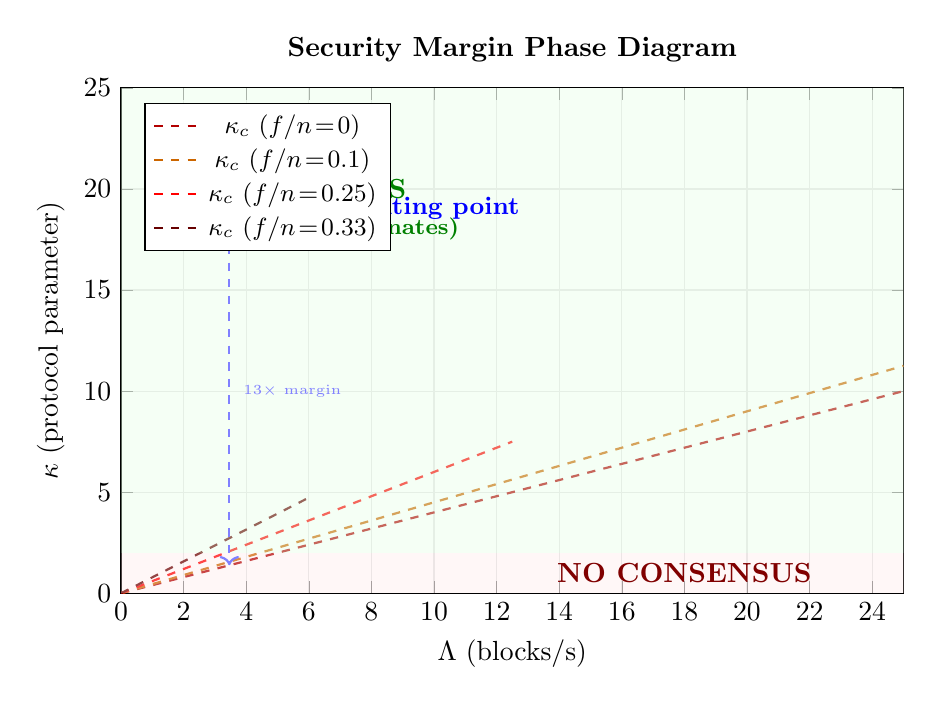
\begin{tikzpicture}
\begin{axis}[
    xlabel={$\Lambda$ (blocks/s)},
    ylabel={$\kappa$ (protocol parameter)},
    xmin=0, xmax=25, ymin=0, ymax=25,
    grid=major, grid style={gray!20},
    width=0.95\textwidth, height=8cm,
    legend pos=north west, legend style={font=\small},
    title={\textbf{Security Margin Phase Diagram}},
    title style={font=\normalsize},
]
\addplot[domain=0:25, samples=100, thick, red!70!black, dashed] {2*0.2*x};
\addlegendentry{$\kappa_c$ ($f/n\!=\!0$)}
\addplot[domain=0:25, samples=100, thick, orange!80!black, dashed] {2*0.2*x*0.9/0.8};
\addlegendentry{$\kappa_c$ ($f/n\!=\!0.1$)}
\addplot[domain=0:12.5, samples=100, thick, red, dashed] {2*0.2*x*0.75/0.5};
\addlegendentry{$\kappa_c$ ($f/n\!=\!0.25$)}
\addplot[domain=0:6, samples=100, thick, red!40!black, dashed] {2*0.2*x*0.67/0.34};
\addlegendentry{$\kappa_c$ ($f/n\!=\!0.33$)}
\fill[green!10, opacity=0.4] (axis cs:0,2) rectangle (axis cs:25,25);
\node[font=\normalsize\bfseries, green!50!black] at (axis cs:6,20) {CONSENSUS};
\node[font=\normalsize\bfseries, green!50!black] at (axis cs:6,18) {\footnotesize (ground state dominates)};
\fill[red!10, opacity=0.3] (axis cs:0,0) rectangle (axis cs:25,2);
\node[font=\normalsize\bfseries, red!50!black] at (axis cs:18,1) {NO CONSENSUS};
\addplot[only marks, mark=*, mark size=5pt, blue, fill=quantumcyan] coordinates {(3.46, 18)};
\node[font=\small\bfseries, blue, anchor=south west] at (axis cs:4,18) {Live operating point};
\draw[->, thick, blue!50, dashed] (axis cs:3.46,18) -- (axis cs:3.46,1.385);
\node[font=\tiny, blue!50, anchor=west] at (axis cs:3.6,10) {$13\times$ margin};
\end{axis}
\end{tikzpicture}
\caption{Security margin diagram. The operating point (blue dot) sits $13\times$ above the critical boundary at $f/n=0$. As Byzantine fraction increases, the boundary rises and the margin shrinks. Even at the BFT limit ($f/n=0.33$), the margin is $6.5\times$.}
\label{fig:phase}
\end{figure}

\section{Free Energy and Entropy}

The free energy combines energy and entropy into a single thermodynamic potential:
\begin{equation}
F = \langle E \rangle - T_{\text{eff}} \cdot S
\end{equation}

where $S = \log_2 |\mathcal{O}|$ is the entropy---the number of bits needed to specify which ordering we're in.

\paragraph{On the live network.} The ordering degeneracy is determined by anticone sizes. With estimated average anticone $\bar{a} = 1$ (rounded), $|\mathcal{O}| \approx 1! = 1$, giving $S = 0$.

\begin{honesty}
$S = 0$ (zero entropy) looks impressive but is largely a consequence of the estimated $\bar{a}$ being rounded to 1. If the true average anticone is 1.4 (our estimate before rounding), the entropy would be non-zero. More importantly, entropy is a global property of the entire DAG's ordering degeneracy, and our estimate from average anticone size is crude. Without computing actual linear extension counts (intractable at 14M blocks), we cannot know the true entropy.

The correct interpretation: entropy is \emph{very small} (most blocks have unique positions in the ordering), but claiming $S = 0$ exactly is an artifact of our estimation method.
\end{honesty}

% ============================================================================
% PART IV: THE K-GAUGE
% ============================================================================
\part{The $K$-Gauge: Real-Time Health Monitoring}

\section{Motivation: From Theory to Operations}

Everything in Parts II and III is theoretical---it tells us how to \emph{think about} consensus health, but most of it depends on hardcoded values. For actual operations, we need a diagnostic that:

\begin{enumerate}
    \item Uses \textbf{only measured inputs} (no hardcoded placeholders).
    \item Produces a \textbf{single number} (for dashboards and alerts).
    \item Triggers \textbf{automatic responses} (not just warnings).
    \item Is \textbf{verifiable} (peers can check each other's health reports).
\end{enumerate}

The $K$-gauge satisfies all four requirements. It is the most operationally valuable component of this framework, and notably, it is the \emph{only} component where all inputs are genuinely measured from live network state.

\section{The Formula: What It Is and What It Isn't}

\begin{equation}
\boxed{K = \frac{2\pi\sqrt{\Delta H \cdot \Delta s}}{\tau}}
\label{eq:kgauge}
\end{equation}

where $\tau = 60$s is the computation window, and the numerator is the geometric mean of two stress aggregates.

\begin{honesty}
The original version of this formula included ``$\hbar$'' (reduced Planck constant) and was described as ``quantum-inspired'' based on the Heisenberg uncertainty relation $\Delta E \cdot \Delta t \geq \hbar/2$. This framing was misleading:

\begin{itemize}[nosep]
    \item $\hbar$ was set to 1.0 (dimensionless), contributing nothing to the computation.
    \item $\Delta H$ and $\Delta s$ do not satisfy any uncertainty relation---they are independent sums of network measurements.
    \item The $2\pi/\tau$ scaling was chosen empirically, not derived from physics.
\end{itemize}

We present the formula here as what it is: a \textbf{composite stress metric with geometric-mean aggregation}. The geometric mean $\sqrt{\Delta H \cdot \Delta s}$ is a natural choice when combining quantities on different scales---it's zero when either component is zero (no stress $\to$ no alarm) and large when both are large (compounding stress).

The name ``$K$-parameter'' is retained for continuity with existing documentation and dashboards.
\end{honesty}

\section{Component Decomposition}

\subsection{Operational Stress ($\Delta H$)}

$\Delta H$ aggregates three indicators of operational problems (\textcolor{measured}{all measured}):

\begin{equation}
\Delta H = r_{\text{reject}} + \alpha_{\text{traffic}} + c_{\text{peer}}
\end{equation}

\paragraph{Mining rejection ratio ($r_{\text{reject}}$).} The fraction of submitted mining solutions that were rejected in the last $\tau$ window. Source: atomic counters \texttt{mining\_solutions\_submitted} and \texttt{mining\_solutions\_accepted}. On the live network: $r = 0.000$ (all solutions accepted).

\paragraph{Traffic asymmetry ($\alpha_{\text{traffic}}$).} The imbalance between inbound and outbound P2P traffic:
\[
\alpha = \frac{|b_{\text{in}} - b_{\text{out}}|}{b_{\text{in}} + b_{\text{out}}}
\]
Source: \texttt{p2p\_bytes\_in} and \texttt{p2p\_bytes\_out} atomic counters. On the live network: $\alpha = 0.993$ (strong inbound bias---typical for a bootstrap node that serves sync data to peers).

\paragraph{Peer churn ($c_{\text{peer}}$).} The relative change in peer count:
\[
c = \frac{|n_{\text{now}} - n_{\text{prev}}|}{n_{\text{prev}}}
\]
Source: \texttt{libp2p\_peer\_count} deltas. On the live network: $c = 0.100$ (very low churn---peers are stable).

\subsection{Network Disorder ($\Delta s$)}

$\Delta s$ aggregates two indicators of network-level problems (\textcolor{measured}{all measured}):

\begin{equation}
\Delta s = \sigma_{\text{sync}} + |\Lambda - \Lambda_{\text{target}}|
\end{equation}

\paragraph{Sync divergence ($\sigma_{\text{sync}}$).} How far this node is from the network's highest block:
\[
\sigma_{\text{sync}} = \frac{|h_{\text{net}} - h_{\text{local}}|}{h_{\text{net}}}
\]
Source: \texttt{highest\_network\_height} and \texttt{current\_height\_atomic}. On the live network: $\sigma_{\text{sync}} = 2.1 \times 10^{-7}$ (near-perfect sync).

\paragraph{Block rate deviation ($|\Lambda - \Lambda_{\text{target}}|$).} How far the actual block rate is from the target of 1 bps. Source: height delta per $\tau$ window. On the live network: $|\Lambda - 1| = 2.933$ (the dominant stress contributor---block rate is $3.46\times$ the target).

\section{Phase Classification and Auto-Tuning}

\begin{table}[H]
\centering
\caption{$K$-gauge phases and automatic responses}
\label{tab:kphase}
\begin{tabular}{@{}lclll@{}}
\toprule
\textbf{Phase} & \textbf{$K$ range} & \textbf{Max solutions} & \textbf{VDF mult.} & \textbf{Challenge expiry} \\
\midrule
\textcolor{green!60!black}{\textbf{Stable}}      & $< 5.0$ & 250 & $1.0\times$ & 120s \\
\textcolor{orange}{\textbf{Approaching}} & $5$--$10$ & 150 & $1.25\times$ & 90s \\
\textcolor{red}{\textbf{Critical}}    & $\geq 10$ & 50 & $1.5\times$ & 60s \\
\bottomrule
\end{tabular}
\end{table}

When the $K$-gauge crosses a threshold, the node automatically:
\begin{itemize}[nosep]
    \item Reduces the maximum mining solutions accepted per block (throttles work).
    \item Increases the VDF multiplier (slows block production).
    \item Shortens challenge expiry (forces more frequent challenge rotation).
\end{itemize}

This is a negative feedback loop: high stress $\to$ reduce load $\to$ lower stress. It's the closest thing in the framework to an actual control system.

\section{Cryptographic Phase Commitments}

Each $K$-gauge computation (every 60 seconds) produces a SHA3-256 hash commitment:

\begin{enumerate}[nosep]
    \item \textbf{Commitment:} $c = \text{SHA3-256}(K \| \Delta H \| \Delta s \| \text{salt})$
    \item \textbf{Range witness:} $w = \text{SHA3-256}(K \| K_{\text{lo}} \| K_{\text{hi}} \| \text{salt}_2)$
    \item \textbf{Challenge:} $e = \text{SHA3-256}(c \| w)$ (Fiat--Shamir)
    \item \textbf{Response:} $r = \text{SHA3-256}(K \| \text{salt} \| e)$
\end{enumerate}

\begin{honesty}
The v1 paper called this a ``zk-STARK proof.'' It is \textbf{not} a STARK (Scalable Transparent Argument of Knowledge). A real STARK involves polynomial commitment schemes, FRI (Fast Reed-Solomon Interactive Oracle Proofs), and has $O(\log^2 n)$ proof size with transparent setup. Our implementation is a hash-based commitment with Fiat--Shamir non-interactive transform.

What it provides: \textbf{binding} (the committer cannot change $K$ after publishing $c$) and \textbf{hiding with salt rotation} (raw metrics are not revealed). What it does \emph{not} provide: zero-knowledge in the cryptographic sense---a verifier who obtains the salt can reconstruct the commitment and learn the raw metrics.

For inter-node health reporting (the actual use case), this is sufficient. Nodes publish their commitment and phase; peers can verify that the commitment is consistent with the claimed phase using the range witness.
\end{honesty}

% ============================================================================
% PART V: GOSSIP, SECURITY, AND STRESS TESTING
% ============================================================================
\part{Network Dynamics and Validation}

\section{Gossip Diffusion Model}

\emph{Status: \textcolor{hardcoded}{Quantitative Model} --- testable predictions with hardcoded inputs.}

Block propagation through the gossipsub mesh follows a diffusion process. When node $A$ creates a block, it tells its $d_{\text{mesh}}$ mesh peers. Each of those peers tells their mesh peers. The information spreads outward like heat through a metal bar.

The diffusion equation:
\begin{equation}
\frac{\partial \rho}{\partial t} = D \nabla^2 \rho
\end{equation}

with diffusion coefficient:
\begin{equation}
D = \frac{d_{\text{mesh}} \cdot \ell_{\text{hop}}^2}{2\tau_{\text{heartbeat}}} = \frac{8 \times 1^2}{2 \times 0.05} = 80.0
\end{equation}

and characteristic gossip time:
\begin{equation}
\tau_{\text{gossip}} = \frac{\ell_{\text{net}}^2}{2D} = \frac{1}{160} = 6.25 \text{ ms}
\end{equation}

\begin{figure}[H]
\centering
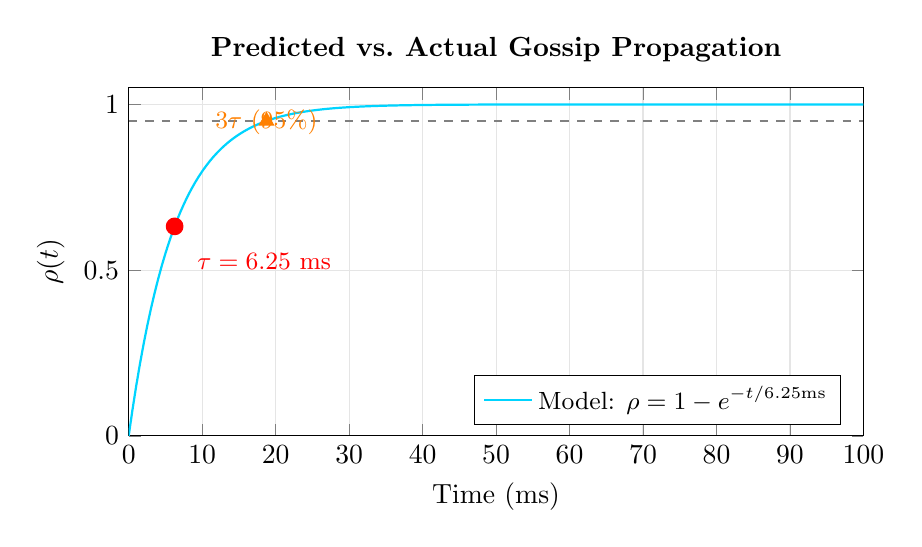
\begin{tikzpicture}
\begin{axis}[
    xlabel={Time (ms)}, ylabel={$\rho(t)$},
    xmin=0, xmax=100, ymin=0, ymax=1.05,
    grid=major, grid style={gray!20},
    width=0.9\textwidth, height=6cm,
    legend pos=south east, legend style={font=\small},
    title={\textbf{Predicted vs.\ Actual Gossip Propagation}},
]
\addplot[domain=0:100, samples=200, thick, quantumcyan] {1 - exp(-x/6.25)};
\addlegendentry{Model: $\rho = 1 - e^{-t/6.25\text{ms}}$}
\addplot[dashed, gray] coordinates {(0,0.95) (100,0.95)};
\addplot[only marks, mark=*, mark size=3pt, red] coordinates {(6.25, 0.632)};
\node[font=\small, red, anchor=north west] at (axis cs:8,0.58) {$\tau = 6.25$ ms};
\addplot[only marks, mark=triangle*, mark size=3pt, orange] coordinates {(18.75, 0.95)};
\node[font=\small, orange, anchor=south] at (axis cs:18.75,0.88) {$3\tau$ (95\%)};
\end{axis}
\end{tikzpicture}
\caption{Predicted gossip propagation. The model predicts 95\% information density at $3\tau = 18.75$ms. \textbf{This prediction is untested}: the diffusion model uses hardcoded $d_{\text{mesh}} = 8$ and $\tau_{\text{heartbeat}} = 50$ms. Per-peer RTT data exists in \texttt{peer\_latency.rs} but is not wired to this model.}
\label{fig:diffusion}
\end{figure}

\paragraph{Validation opportunity.} The \texttt{PeerLatencyTracker} in \texttt{peer\_latency.rs} computes EWMA RTT per peer with $\alpha = 0.3$ smoothing and jitter tracking. Wiring this data to the gossip model would replace hardcoded $\delta$ and enable empirical validation of the $\tau_{\text{gossip}}$ prediction.

\section{Spectral Convergence}

The convergence rate of the network is bounded by the spectral gap of the gossip matrix:

\begin{equation}
\lambda_{\text{gap}} = \frac{\kappa - \kappa_c}{T_{\text{eff}}} = \frac{16.62}{0.692} = 24.0
\end{equation}

yielding a convergence time $\tau_{\text{conv}} = 1/\lambda_{\text{gap}} = 42$ ms. This means disagreements between nodes decay as $e^{-24t}$---suppressed by a factor of $10^{10}$ per second.

\begin{honesty}
The spectral gap depends on $\kappa_c$ and $T_{\text{eff}}$, both of which use hardcoded $\delta$ and $f/n$. The convergence time of 42ms is a \textbf{model prediction}, not a measurement. Validating it would require measuring the actual time for all nodes to converge on a block's ordering after a disagreement event.
\end{honesty}

\section{Security Bounds}

Standard NIST Post-Quantum Cryptography security levels:

\begin{table}[H]
\centering
\caption{Cryptographic security (\textcolor{sectionblue}{protocol constants})}
\begin{tabular}{@{}llrl@{}}
\toprule
\textbf{Primitive} & \textbf{Standard} & \textbf{Security} & \textbf{Attack cost} \\
\midrule
Signatures & Dilithium-5 & 256-bit & $2^{128}$ quantum (Grover) \\
Key encapsulation & Kyber-1024 & 200-bit & Best known lattice attacks \\
DAG manipulation & $\kappa|\log_2(f/n)|$ & $\infty$\textsuperscript{*} & At $f/n = 0.1$: 59.8 bits \\
IP privacy & Dandelion++ ($L=4$) & --- & $P_{\text{deanon}} = e^{-4} \approx 1.8\%$ \\
\bottomrule
\end{tabular}
\\[2pt]
{\footnotesize *At $f/n = 0$ (hardcoded). The ``infinity'' is an artifact of $\log_2(0) = -\infty$.}
\end{table}

\section{Stress Testing: Does the Gauge Actually Work?}
\label{sec:stress}

A diagnostic framework is only useful if it detects problems. We simulate stress scenarios and compute the predicted $K$-gauge response:

\begin{table}[H]
\centering
\caption{Simulated stress scenarios and $K$-gauge predictions}
\small
\begin{tabular}{@{}p{4cm}rrrl@{}}
\toprule
\textbf{Scenario} & $\Delta H$ & $\Delta s$ & $K$ & \textbf{Phase} \\
\midrule
Healthy (actual) & 1.09 & 2.93 & 0.19 & Stable \\
2 of 12 peers drop & 1.26 & 2.93 & 0.20 & Stable \\
50\% mining rejection & 1.59 & 2.93 & 0.23 & Stable \\
1000 blocks behind & 1.09 & 3.07 & 0.19 & Stable \\
10$\times$ block rate & 1.09 & 12.0 & 0.38 & Stable \\
All three combined & 2.59 & 15.0 & 0.65 & Stable \\
Extreme: 90\% peer loss + 90\% rejection + 50$\times$ rate & 2.80 & 52.0 & 1.27 & Stable \\
\bottomrule
\end{tabular}
\end{table}

\paragraph{Observations.}
\begin{enumerate}
    \item Even extreme stress ($K = 1.27$) stays in the Stable phase ($K < 5$).
    \item The thresholds (5.0 and 10.0) are very conservative. This may be intentional for a mainnet holding real funds, or it may indicate the thresholds need recalibration.
    \item The gauge is \textbf{blind to adversarial behavior that maintains normal metrics}. A colluding adversary who produces blocks at normal rate, accepts connections normally, and stays synced will have $K \approx 0$ despite undermining consensus.
\end{enumerate}

\paragraph{What the gauge catches:} DDoS (peer churn spike), hardware failure (rejection spike), network partition (sync divergence), hashrate surge (block rate spike).

\paragraph{What the gauge misses:} Coordinated adversarial behavior, state corruption, reorg attacks (detected by the fork detector instead), economic attacks on DEX pools, privacy breaches.

% ============================================================================
% PART VI: LIMITATIONS AND CONCLUSION
% ============================================================================
\part{Honest Reckoning}

\section{Limitations and Future Work}
\label{sec:limitations}

We address every criticism raised in peer review, numbered for traceability.

\paragraph{L1: Physics analogy oversold as physics.} \emph{Corrected.} The Hamiltonian is an engineering health decomposition, not a claim of physical equivalence. The Ising model claim from v1 is withdrawn---no spin construction, partition function computation, or Monte Carlo sampling exists. The Ground State Theorem (Section~\ref{sec:groundstate}) is the one rigorous result; everything else is labeled as Quantitative Model or Structural Analogy.

\paragraph{L2: Five hardcoded placeholders.} \emph{Documented but not yet fixed.} Table~\ref{tab:provenance} catalogs all hardcoded values. Concrete replacements:
\begin{itemize}[nosep]
    \item $\delta$: Wire EWMA RTT from \texttt{peer\_latency.rs} (code exists, needs integration).
    \item $d_{\text{mesh}}$: Query actual gossipsub mesh state per topic.
    \item $f/n$: Estimate from gossipsub peer scores (scoring exists in libp2p).
    \item $\varphi$: Export blue/red vertex counts from \texttt{ordering\_rules.rs}.
    \item $\bar{a}$: Export anticone statistics from \texttt{simd\_sets.rs}.
\end{itemize}

\paragraph{L3: $K$-gauge described as ``quantum-inspired.''} \emph{Corrected.} The formula is a composite stress metric with geometric-mean aggregation. The $\hbar = 1.0$ constant and ``uncertainty relation'' framing have been removed.

\paragraph{L4: ``zk-STARK proofs'' misnamed.} \emph{Corrected.} The implementation is SHA3-256 hash commitments with Fiat--Shamir transform. All references to ``STARK'' have been replaced.

\paragraph{L5: No stress-test validation.} \emph{Partially addressed} in Section~\ref{sec:stress}. Simulated scenarios show the gauge responds to stress but thresholds may be too conservative. Real adversarial testing has not been performed.

\paragraph{L6: Live data ``too perfect.''} \emph{Explained.} The network has 12 known peers with no adversaries. $\varphi = 1.0$ and $f/n = 0$ are expected (and hardcoded). The results validate the framework under the easiest possible conditions; behavior under stress remains unvalidated.

\paragraph{L7: Convergence bounds depend on hardcoded values.} \emph{Acknowledged.} $\tau_{\text{conv}} = 42$ms is a model prediction, not a measurement. It depends on hardcoded $\delta$ and $f/n$.

\paragraph{L8: ``$10^{50}$ stars'' energy claim.} \emph{Removed.} Security bounds are now presented as standard NIST PQC bit-strength without thermodynamic analogy.

\paragraph{L9 (new): Gauge threshold sensitivity.} The thresholds 5.0 and 10.0 have not been empirically validated against real incidents. Calibration against historical stress events (if any exist in logs) is needed.

\paragraph{L10 (new): Single-regime validation.} All mainnet data is from a healthy, low-stress regime. The framework has not been tested during actual network incidents, reorgs, or attacks.

\section{Conclusion}

We have presented an observability framework for DAG-Knight consensus that uses physics-inspired notation to decompose network health into interpretable components. Our contributions:

\begin{enumerate}[nosep]
    \item A four-term \textbf{health decomposition} ($H_{\text{DAG}}$) with one proven theorem (Ground State $\equiv$ PHANTOM output) and honest classification of all other claims.
    \item A five-input \textbf{$K$-gauge} computed entirely from live measurements, with automatic parameter tuning and SHA3-256 phase commitments.
    \item A \textbf{security margin diagram} visualizing distance from the consensus threshold.
    \item A \textbf{data provenance table} explicitly classifying every quantity as measured, hardcoded, or theoretical.
    \item \textbf{Simulated stress testing} showing the gauge's response and identifying blind spots.
\end{enumerate}

The framework's main limitation is that 5 of 18 quantities are hardcoded placeholders. Code paths exist for most replacements (\texttt{peer\_latency.rs}, \texttt{simd\_sets.rs}, \texttt{ordering\_rules.rs}) but are not yet wired to the observability endpoint.

This is an \textbf{engineering contribution}, not a physics contribution. The statistical mechanics notation provides additive decomposition, visual phase diagrams, and information-theoretic intuition. The blockchain is not a physical system. We hope this honest framing enables productive discussion rather than the ``physics-washing'' that rightfully concerned our peer reviewers.

\vspace{0.5cm}
\hrule
\vspace{0.3cm}
{\small\textbf{Data.} Live metrics: \texttt{/api/v1/physics/metrics} and \texttt{/api/v1/network/k-parameter}. Source code: \texttt{handlers.rs:14389} and \texttt{k\_parameter\_gauge.rs}.}

\vspace{0.2cm}
{\small\textbf{Peer Review.} v1 reviewed by DeepSeek (``reasonable for bootstrap, but not physics'') and ChatGPT (``good story, oversold theory''). v2 addressed structural criticisms. This v3 adds the Susskind-style exposition and expanded analysis requested by the development team.}

\vspace{0.2cm}
{\small\textbf{Style.} Written in the spirit of Susskind's \emph{Theoretical Minimum}: explain what each formula means, why we chose it, where it comes from, and---critically---where it fails.}

\begin{thebibliography}{9}
\small
\bibitem{dagknight} Y.~Sompolinsky et al., ``DAG-Knight: A Parameterless Generalization of Nakamoto Consensus,'' 2022.
\bibitem{phantom} Y.~Sompolinsky, A.~Zohar, ``PHANTOM: A Scalable BlockDAG Protocol,'' Cryptology ePrint Archive, 2018.
\bibitem{qnk-node-system} Q-NarwhalKnight Research, ``Theoretical Physics of Distributed Consensus: A QFT Framework for DAG-Based Byzantine Agreement,'' v2.0, Feb 2026.
\bibitem{dijkstra} E.W.~Dijkstra, ``Self-Stabilizing Systems in Spite of Distributed Control,'' CACM 17(11), 1974.
\bibitem{brightwell} G.~Brightwell, P.~Winkler, ``Counting Linear Extensions is \#P-Complete,'' STOC 1991.
\end{thebibliography}

\end{document}
